%%
%% Modified by Ricardo Garcia-Rosas to satisfy the rules established by the University of Melbourne's Research Higher Degrees Committee as of 4th of June 2019.
%% Guidelines can be found at: https://gradresearch.unimelb.edu.au/__data/assets/pdf_file/0004/2027839/Preparation-of-GR-theses-rules.pdf
%%
%%%%%%%%%%%%%%%%%%%%%%%%%%%%%%%%%%%%%%%%%%%%%%%%%%%%%%%%%%%%%%%%%%%%%%%%%
%% IMPORTANT NOTE TO AUTHOR:
%% As part of the guidelines, the use of the university logo is not permitted. This template contains it to make it easier to find/recognise in the Overleaf Gallery. To make the template compliant please go to 'Thesis.cls' and comment out the \includegraphics command in line 217 (it is clearly highlited).
%%%%%%%%%%%%%%%%%%%%%%%%%%%%%%%%%%%%%%%%%%%%%%%%%%%%%%%%%%%%%%%%%%%%%%%%%
%%
%% ----------------------------------------------------------------
%% Thesis.tex -- MAIN FILE (the one that you compile with LaTeX)
%% ---------------------------------------------------------------- 

% Set up the document
\documentclass[a4paper, 12pt, oneside]{Thesis}  % Use the "Thesis" style, based on the ECS Thesis style by Steve Gunn
%
% Put your figures in this directory
\graphicspath{Figures/}  % Location of the graphics files (set up for graphics to be in PDF format)
%

% Include any extra LaTeX packages required
\usepackage[square, numbers, comma, sort&compress]{natbib}  % Use the "Natbib" style for the references in the Bibliography
\usepackage{verbatim}  % Needed for the "comment" environment to make LaTeX comments
\usepackage{vector}  % Allows "\bvec{}" and "\buvec{}" for "blackboard" style bold vectors in maths
\hypersetup{urlcolor=blue, colorlinks=true}  % Colours hyperlinks in blue, but this can be distracting if there are many links.

%% ----------------------------------------------------------------
\begin{document}
\frontmatter      % Begin Roman style (i, ii, iii, iv...) page numbering

%
\UNIVERSITY{{THE UNIVERSITY OF MELBOURNE }}    
%
%%%%%%%%%%%%%%%%%%%%%%%%%%%%%%%%%%%%%%%%%%%%%%%%%%%%%%%%%%%%%%%%%%%%%%%%%
% Update your department and school here:
\department{{Faculty of Science}}
\school{{School of Mathematics and Statistics}}
%%%%%%%%%%%%%%%%%%%%%%%%%%%%%%%%%%%%%%%%%%%%%%%%%%%%%%%%%%%%%%%%%%%%%%%%%

%
%%%%%%%%%%%%%%%%%%%%%%%%%%%%%%%%%%%%%%%%%%%%%%%%%%%%%%%%%%%%%%%%%%%%%%%%%
% Set up the Title Page
% Change your thesis title and your information here
\title  {The Grothendieck-Teichm\"uller Group and the Operad of Parenthesized Braids}
\authors  {\texorpdfstring
            {\href{https://www.github.com/zin3724}{Yaxin Li}}
            {Yaxin Li}
            }
\addresses  {\groupname\\\deptname\\\univname}  % Do not change this here, instead these must be set in the "Thesis.cls" file, please look through it instead
\date       {\today}
\subject    {}
\keywords   {}
%%%%%%%%%%%%%%%%%%%%%%%%%%%%%%%%%%%%%%%%%%%%%%%%%%%%%%%%%%%%%%%%%%%%%%%%%

\maketitle
%% ----------------------------------------------------------------

% \setstretch{1.3}  % It is better to have smaller font and larger line spacing than the other way round

% Define the page headers using the FancyHdr package and set up for one-sided printing
\fancyhead{}  % Clears all page headers and footers
\rhead{\thepage}  % Sets the right side header to show the page number
\lhead{}  % Clears the left side page header

\pagestyle{fancy}  % Finally, use the "fancy" page style to implement the FancyHdr headers

%% ----------------------------------------------------------------
% The Abstract Page

\addtotoc{Abstract}  % Add the "Abstract" page entry to the Contents
\abstract{
\addtocontents{toc}{\vspace{1em}}  % Add a gap in the Contents, for aesthetics

We introduce the operad of parenthesized braids $\PaB$, show that algebras over $\PaB$ correspond to braided monoidal categories, and describe the action of the Grothendieck-Teichm\"uller group $\GT$ on $\PaB$.
% (which comes from the $\GT$-action on Drinfeld associators)

}
\clearpage  % Abstract ended, start a new page

%% ----------------------------------------------------------------
% Declaration Page required for the Thesis, your institution may give you a different text to place here
% %
% Guidelines as of 2019/06/04
% https://gradresearch.unimelb.edu.au/__data/assets/pdf_file/0004/2027839/Preparation-of-GR-theses-rules.pdf
%
\Declaration{

\addtocontents{toc}{\vspace{1em}}  % Add a gap in the Contents, for aesthetics

I, Yaxin Li, declare that this thesis titled, `All Star-Autonomous Categories are Coloured Cyclic Operads' and the work presented in it are my own. I confirm that:

\begin{itemize} 
\item[\tiny{$\blacksquare$}] The thesis comprises only my original work towards the MASTER OF SCIENCE except where indicated in the preface;
 
\item[\tiny{$\blacksquare$}] due acknowledgement has been made in the text to all other material used; and

\item[\tiny{$\blacksquare$}] the thesis is fewer than the maximum word limit in length, exclusive of tables, maps, bibliographies and appendices as approved by the Research Higher Degrees Committee.
\\
\end{itemize}
 
 
Signed:\\
\rule[1em]{25em}{0.5pt}  % This prints a line for the signature
 
Date:\\
\rule[1em]{25em}{0.5pt}  % This prints a line to write the date
}
% \clearpage  % Declaration ended, now start a new page

%% ----------------------------------------------------------------
% Preface Page required for the Thesis, your institution may give you a different text to place here
% %
% Guidelines as of 2019/06/04
% https://gradresearch.unimelb.edu.au/__data/assets/pdf_file/0004/2027839/Preparation-of-GR-theses-rules.pdf
%
\Preface{

\addtocontents{toc}{\vspace{1em}}  % Add a gap in the Contents, for aesthetics

Where applicable, the following information must be included in a preface:
\begin{itemize}
\item[\tiny{$\blacksquare$}] a description of work towards the thesis that was carried out in collaboration with others, indicating the nature and proportion of the contribution of others and in general terms the portions of the work which the student claims as original;
\item[\tiny{$\blacksquare$}] a description of work towards the thesis that has been submitted for other qualifications;
\item[\tiny{$\blacksquare$}] a description of work towards the thesis that was carried out prior to enrolment in the degree;
\item[\tiny{$\blacksquare$}] whether any third party editorial assistance was provided in preparation of
the thesis and whether the persons providing this assistance are knowledgeable in the academic discipline of the thesis;
\item[\tiny{$\blacksquare$}] the contributions of all persons involved in any multi-authored publications or
articles in preparation included in the thesis;
\item[\tiny{$\blacksquare$}] the publication status of all chapters presented in article format using the
descriptors below;
    \begin{itemize}
        \item Unpublished material not submitted for publication
        \item Submitted for publication to [publication name] on [date]
        \item In revision following peer review by [publication name]
        \item Accepted for publication by [publication name] on [date]
        \item Published by [publication name] on [date]
    \end{itemize}
\item[\tiny{$\blacksquare$}] an acknowledgement of all sources of funding, including grant identification
numbers where applicable and Australian Government Research Training Program Scholarships, including fee offset scholarships.
\end{itemize}

}
% \clearpage  % Preface ended, now start a new page

%% ----------------------------------------------------------------
% The Acknowledgements page, for thanking everyone
% \setstretch{1.3}  % Reset the line-spacing to 1.3 for body text (if it has changed)
\acknowledgements{
\addtocontents{toc}{\vspace{1em}}  % Add a gap in the Contents, for aesthetics

The acknowledgements and the people to thank go here, don't forget to include your project advisor\ldots

}
\clearpage  % End of the Acknowledgements
%% ----------------------------------------------------------------

\pagestyle{fancy}  %The page style headers have been "empty" all this time, now use the "fancy" headers as defined before to bring them back


%% ----------------------------------------------------------------
\lhead{\emph{Contents}}  % Set the left side page header to "Contents"
\tableofcontents  % Write out the Table of Contents

%% ----------------------------------------------------------------
% \lhead{\emph{List of Figures}}  % Set the left side page header to "List if Figures"
% \listoffigures  % Write out the List of Figures

%% ----------------------------------------------------------------
% \lhead{\emph{List of Tables}}  % Set the left side page header to "List of Tables"
% \listoftables  % Write out the List of Tables

%% ----------------------------------------------------------------
% \setstretch{1.5}  % Set the line spacing to 1.5, this makes the following tables easier to read
\setstretch{2.0}  % Set the line spacing to 2.0
\clearpage  % Start a new page
\lhead{\emph{Abbreviations}}  % Set the left side page header to "Abbreviations"
\listofsymbols{ll}  % Include a list of Abbreviations (a table of two columns)
{
% \textbf{Acronym} & \textbf{W}hat (it) \textbf{S}tands \textbf{F}or \\
\textbf{LAH} & \textbf{L}ist \textbf{A}bbreviations \textbf{H}ere \\

}

%% ----------------------------------------------------------------
% \clearpage  % Start a new page
% \lhead{\emph{Constants}}  % Set the left side page header to "Physical Constants"
% \listofconstants{lrcl}  % Include a list of Physical Constants (a four column table)
% {
% % Constant Name & Symbol & = & Constant Value (with units) \\
% Speed of Light & $c$ & $=$ & $2.997\ 924\ 58\times10^{8}\ \mbox{ms}^{-\mbox{s}}$ (exact)\\

% }

%% ----------------------------------------------------------------
\clearpage  %Start a new page
\lhead{\emph{Symbols}}  % Set the left side page header to "Symbols"

  % Include a list of Symbols (a three column table)
\listofnomenclature{lll}
{
% symbol & name & unit \\
$a$ & distance & m \\
$P$ & power & W (Js$^{-1}$) \\
{}& & \\ % Gap to separate the Roman symbols from the Greek
$\omega$ & angular frequency & rads$^{-1}$ \\
}
%% ----------------------------------------------------------------
% End of the pre-able, contents and lists of things


%% ----------------------------------------------------------------
\mainmatter	  % Begin normal, numeric (1,2,3...) page numbering
\pagestyle{fancy}  % Return the page headers back to the "fancy" style

% Include the chapters of the thesis, as separate files
% Just uncomment the lines as you write the chapters

\chapter{Introduction}
\lhead{\emph{Introduction}}
$\mathcal{M}_{g,n}$ is the moduli stack (i.e. 2-scheme) of genus-$g$ curves over $\bQ$ with $n$ marked points. In his Sketch of a Program \cite{Grothendieck_1997} from 1983, Grothendieck proposes that we study $G_\bQ\defeq\mathrm{Gal}(\overline\bQ/\bQ)$ through its action on the Teichm\"uller Tower --- the collection of
\[\pi^{\mathrm{geom}}_1(\mathcal{M}_{g,n})\defeq\pi_1^{\mathrm{et}}(\overline{\bQ}\times_{\bQ}\mathcal{M}_{g,n})\]
for all $g,n\in\bN$. Here, $\pi_1^{\mathrm{et}}$ takes the \'etale fundamental group, which is the inverse limit of the automorphism groups (analogous to the groups of deck transformations) of finite \'etale covers.

In genus-0, it is known that $\pi^{\mathrm{geom}}_1(\mathcal{M}_{0,4})\cong\widehat{F_2}$, the profinite completion of the free group on two generators. It follows from a theorem of Belyi's \cite{Belyĭ_1980} that $G_\bQ$ acts faithfully on $\pi^{\mathrm{geom}}_1(\mathcal{M}_{0,4})$, hence also $\lt\{\mathcal{M}_{0,n}\rt\}_n$. In \cite{Ihara_1991}, Ihara showed that the image of the action of $G_\bQ$ includes into the image of $\GThat$, the profinite completion of the inertia-preserving automorphisms of $\lt\{\mathcal{M}_{0,n}\rt\}_n$, i.e. the automorphisms $F$ such that on $\widehat{F_2}$, $F$ maps the procyclic subgroups $\lgl x\rgl,\lgl y\rgl,\lgl(xy)^{-1}\rgl$ to conjugate subgroups, where $x$ and $y$ are the generators of $F_2$ \cite{Lochak}.

In \cite{Drinfeld_1991}, Drinfeld constructs a pro-unipotent
% todo: if there is room, describe in a few sentences
version of $\GT$, and uses its action on braided monoidal categories (i.e. $\PaBhat$-algebras) to prove a result about quasitriangular quasi-Hopf algebras.
% todo: if there is room, insert short rant about deformation quantization and Drinfeld associators?
In \cite{Petersen_2014}, Petersen uses the corresponding action on $\PaBhat$ to show that $E_2$ (the operad of little 2-disks) is formal. % Introduction

%\chapter{\texorpdfstring{Algebras of $\PaB$}{Algebras of PaB}}
\lhead{\emph{algebras of $\PaB$}}
\section{Braided Monoidal Categories}
\begin{definition}[monoidal category]
	A category $\sC$ with a bifunctor $-\otimes-:\sC\times\sC\to\sC$ (the monoidal, or tensor product), unit object $\mathbf{1}$, and natural isomorphisms
	\begin{align}
		&\alpha:(-\otimes-)\otimes-\Rightarrow-\otimes(-\otimes-)\\
		&\lambda:\mathbf{1}\otimes-\Ra\id_\sC & \rho:-\otimes\mathbf{1}\Ra\id_{sC}
	\end{align}
	 respectively called the associator, left unitor, right unitor, is \emph{monoidal} if when we write $\otimes$ to act componentwise on natural transformations,
	\begin{enumerate}
	\item the triangle identity is satisfied, i.e. $\rho\otimes\id_\sC=(\id_\sC\otimes\lambda)\circ\alpha$
	\item the pentagon identity holds, i.e. for all $w,x,y,z\in\Obj(\sC)$, the following diagram commutes
	

\tikzset{every picture/.style={line width=0.75pt}} %set default line width to 0.75pt        
\[
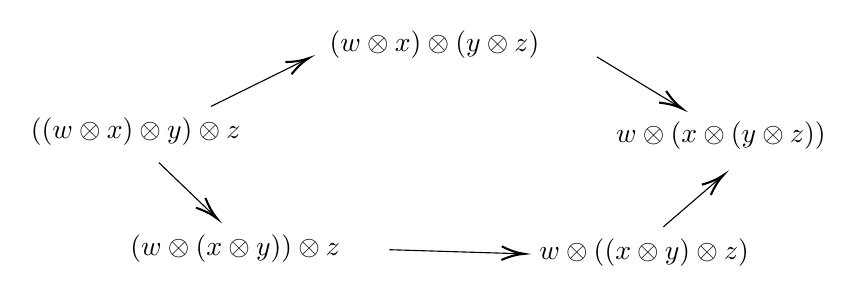
\begin{tikzpicture}[x=0.75pt,y=0.75pt,yscale=-1,xscale=1]
%uncomment if require: \path (0,497); %set diagram left start at 0, and has height of 497

%Straight Lines [id:da8091689343428804] 
\draw    (162,295.1) -- (207.41,272.69) ;
\draw [shift={(209.2,271.8)}, rotate = 153.73] [color={rgb, 255:red, 0; green, 0; blue, 0 }  ][line width=0.75]    (10.93,-3.29) .. controls (6.95,-1.4) and (3.31,-0.3) .. (0,0) .. controls (3.31,0.3) and (6.95,1.4) .. (10.93,3.29)   ;
%Straight Lines [id:da5599598183630712] 
\draw    (348,271.2) -- (387.29,295.06) ;
\draw [shift={(389,296.1)}, rotate = 211.27] [color={rgb, 255:red, 0; green, 0; blue, 0 }  ][line width=0.75]    (10.93,-3.29) .. controls (6.95,-1.4) and (3.31,-0.3) .. (0,0) .. controls (3.31,0.3) and (6.95,1.4) .. (10.93,3.29)   ;
%Straight Lines [id:da8391035848401762] 
\draw    (137,322.2) -- (163.56,347.71) ;
\draw [shift={(165,349.1)}, rotate = 223.85] [color={rgb, 255:red, 0; green, 0; blue, 0 }  ][line width=0.75]    (10.93,-3.29) .. controls (6.95,-1.4) and (3.31,-0.3) .. (0,0) .. controls (3.31,0.3) and (6.95,1.4) .. (10.93,3.29)   ;
%Straight Lines [id:da28460978615375354] 
\draw    (248,364.1) -- (311,366.04) ;
\draw [shift={(313,366.1)}, rotate = 181.76] [color={rgb, 255:red, 0; green, 0; blue, 0 }  ][line width=0.75]    (10.93,-3.29) .. controls (6.95,-1.4) and (3.31,-0.3) .. (0,0) .. controls (3.31,0.3) and (6.95,1.4) .. (10.93,3.29)   ;
%Straight Lines [id:da9551788148488187] 
\draw    (380,353.1) -- (407.49,329.41) ;
\draw [shift={(409,328.1)}, rotate = 139.24] [color={rgb, 255:red, 0; green, 0; blue, 0 }  ][line width=0.75]    (10.93,-3.29) .. controls (6.95,-1.4) and (3.31,-0.3) .. (0,0) .. controls (3.31,0.3) and (6.95,1.4) .. (10.93,3.29)   ;

% Text Node
\draw (74,299.4) node [anchor=north west][inner sep=0.75pt]    {$(( w\otimes x) \otimes y) \otimes z$};
% Text Node
\draw (218,257.4) node [anchor=north west][inner sep=0.75pt]    {$( w\otimes x) \otimes ( y\otimes z)$};
% Text Node
\draw (356,301.4) node [anchor=north west][inner sep=0.75pt]    {$w\otimes ( x\otimes ( y\otimes z))$};
% Text Node
\draw (122,355.4) node [anchor=north west][inner sep=0.75pt]    {$( w\otimes ( x\otimes y)) \otimes z$};
% Text Node
\draw (319,357.4) node [anchor=north west][inner sep=0.75pt]    {$w\otimes (( x\otimes y) \otimes z)$};


\end{tikzpicture}
\]
	or as natural transformations, $\alpha\circ\alpha=(\id_\sC\otimes\alpha)\circ\alpha\circ(\alpha\otimes\id_\sC)$
	\end{enumerate}
\end{definition}

A monoidal category is \emph{strict} if the components of the associator and unitors are identity morphisms.
\begin{definition}[braided monoidal category] \label{braidedMonoidalCategory}
	If $(\sC,\otimes,\mathbf{1},\alpha,\lambda,\rho)$ is a monoidal category with a natural isomorphism $\beta_{x,y}:x\otimes y\to y\otimes x$, then it is \emph{braided} if it satisfies the hexagon identities, i.e. the following diagrams commute
	\[
\begin{tikzcd}
	% https://tikzcd.yichuanshen.de/#N4Igdg9gJgpgziAXAbVABwnAlgFyxMJZABgBpiBdUkANwEMAbAVxiRAAoAPAHW4jwC28AAQBPAJS9+WIXGEAvEAF9S6TLnyEUARnJVajFmx59B8dqKlm588ctUgM2PASIAmPdXrNWiDpdMZEVsrILlOezVnTSIybX1vIz8LUNlhTklAtMUVKI1XHVJ4r0NfEADpWS5U4Ltcx3UXLWQPYoMfNgrrdnka8Lr9GCgAc3giUAAzACcIASQyEBwIJABmEo6-XgAjGBw6Pt4sKAB9XjgAYRBqBjodhgAFRpi-BhgJnEiQadn56iWkXTtJIgXiMNAACzoVxANzuj2iBRhbw+9W+c0QgP+iA8QLK212UOutxgDyeiNe70+aKQOKxAFZ1sDQQwIYSYcTSQitEjKaiZui1otlogACyMvHcMGQ6Gwknw-LcikohzU0V-YUM9lwsmK5HQxISo6nbgXA7cHZ7ZQUJRAA
(x\otimes y)\otimes z \arrow[d, "\beta\otimes\id_\sC"] \arrow[r, "\alpha"] & x\otimes(y\otimes z) \arrow[r, "\beta"]               & (y\otimes z)\otimes x \arrow[d, "\alpha"] \\
(y\otimes x)\otimes z \arrow[r, "\alpha"]                                  & y\otimes(x\otimes z) \arrow[r, "\id_\sC\otimes\beta"] & y\otimes(z\otimes x)                     
\end{tikzcd}\]
	\[
\begin{tikzcd}
	% https://tikzcd.yichuanshen.de/#N4Igdg9gJgpgziAXAbVABwnAlgFyxMJZABgBpiBdUkANwEMAbAVxiRAA8AdTiPAW3gAKAJ7deWAXAAEALwCUIAL6l0mXPkIoAjOSq1GLNoK49+8KcLliz0mUpUgM2PASIAmXdXrNWiEDOsJIRNxSQsFZVVnDXdSLT1vQz9BANMg6XYrNLDheyj1VxQyeK8DXw5AyRTK80s8xzUXTWQdEv0fIxCbWSzQ2qU9GCgAc3giUAAzACcIPiQyEBwIJB12pJBuRjQACzoAPWAAWi1FeunZleolpA818u4AIxgcOjOZucRb68QAZlKOvybBg7fZHE5vC6IBbfAAs-3W3CwUAA+tw4ABhGpwR7PV6REDnD5wxbLRAAVnh904W12B2Op3xhKQFJJSD+dzYOJeWMRKLR6IGiiAA
x\otimes(y\otimes z) \arrow[r, "\alpha^{-1}"] \arrow[d, "\id_\sC\otimes\beta"] & (x\otimes y)\otimes z \arrow[r, "\beta"]               & z\otimes(x\otimes y) \arrow[d, "\alpha^{-1}"] \\
x\otimes(z\otimes y) \arrow[r, "\alpha^{-1}"]                                  & (x\otimes z)\otimes y \arrow[r, "\beta\otimes\id_\sC"] & (z\otimes x)\otimes y                        
\end{tikzcd}\]
\end{definition}

We will now build up to Mac Lane's Coherence Theorem
\begin{definition}[monoidal functor, or strong monoidal functor at nLab]
	Suppose $(\sC,\otimes,\mathbf{1},\alpha,\lambda,\rho)$, and $(\sC',\otimes',\mathbf{1}',\alpha',\lambda',\rho')$, are monoidal categories, then a monoidal functor consists of a functor $F:\sC\to\sC'$ such that $\mathbf{1'}\cong F(\mathbf{1})$, and a natural isomorphism $m:F(-)\otimes F(-)\to F(-\otimes-)$ such that the following diagram commutes
	\[\begin{tikzcd}
		% https://tikzcd.yichuanshen.de/#N4Igdg9gJgpgziAXAbVABwnAlgFyxMJZABgBpiBdUkANwEMAbAVxiRAAoAxdgDQEoAOgIh4AtvAAE3AJp9BwsZO4AtPiAC+pdJlz5CKMgEYqtRizbceQkVnFwJs64vsq1m7djwEiZAEwn6ZlZEEG5eJ1tJRwVI+1UNLRAMTz0iQ1J-akDzEMsIu3ZpfMlVN0Tk3W8UdMoss2DQ3nkbAplm5yl2UoSPSv1kdOM6oIsm4pdC8Yl49RMYKABzeCJQADMAJwhRJDIQHAgkdNMRkNFxoSwoAH0hOABhHpANrcPqfaRfYZyQbfcnze2iE+ewOiAAzF8GtwhIw0AALOhlNYAnZvUEAFkhbBhDHhdAA5I9noDMSCkABWLEhC7XW53Ka-RLEilopAQ47fX4UdRAA
(F(X)\otimes F(Y))\otimes F(Z) \arrow[d, "m\otimes\id_\sC"] \arrow[r, "\alpha'"] & F(X)\otimes(F(Y)\otimes F(Z)) \arrow[d, "\id_\sC\otimes m"] \\
F(X\otimes Y)\otimes F(Z) \arrow[d, "m"]                                         & F(X)\otimes F(Y\otimes Z) \arrow[d, "m"]                    \\
F((X\otimes Y)\otimes Z) \arrow[r, "F(\alpha)"]                                  & F(X\otimes(Y\otimes Z))                                    
\end{tikzcd}\]
\end{definition}
A monoidal functor that happens to be an equivalence of categories is called an \emph{equivalence of monoidal categories}.
\begin{theorem}[Mac Lane's Strictness Theorem]
	For any monoidal category\\
	$(\sC,\otimes,\mathbf{1},\alpha,\lambda,\rho)$, there exists a \emph{strict} monoidal category $(\sC',\otimes',\mathbf{1}',\alpha',\lambda',\rho')$ and an equivalence of monoidal categories $L:\sC\to\sC'$.
\end{theorem}
\begin{proof}
	see pg. 20 of \cite{Etingof} from the 2009 lecture notes to "Topics in Lie Theory".
	% Let $\sC'$ be pairs $(F,c)$ where $F$ is an endofunctor of $\sC$, and $c:F(-)\otimes\id_\sC\to F(-\otimes\id_\sC)$ is a natural isomorphism. Then $\sC'$ is strict, and we can construct an equivalence of monoidal categories $L:\sC\to\sC'$ by left multiplication:
	% \begin{enumerate}
	% 	\item For all $X\in\Obj(\sC)$, $L(X)\defeq X\otimes-$.
	% 	\item For morphisms $f$ in $\sC$, $L(f)\defeq f\otimes-$.
	% \end{enumerate}
\end{proof}
The next theorem is a corollary of Mac Lane's Strictness Theorem.
\begin{theorem}[Mac Lane's Coherence Theorem] \label{MacLaneCoherenceThm}
	Suppose $P$ and $P'$ are parenthesizations of $X_1\otimes\cdots\otimes X_n$ with arbitrary insertions of $\mathbf{1}$, and $f,g:P\to P'$ are isomorphisms built by composing associator and unitor components, then $f=g$.
\end{theorem}
\begin{proof}
	see pg. 1 of \cite{Etingof_2009}
\end{proof}

\section{\texorpdfstring{The Operad $\PaB$ of Parenthesized Braids}{The Operad PaB of Parenthesized Braids}}
Operads are an unbiased way of keeping track of $n$-ary operations and how they compose. The "elements" of $P(n)$, we imagine to be corollas, i.e., rooted trees of depth 1 with $n+1$ half-edges. We can treat $\otimes$ in this "unbiased" way (i.e. ignoring how products are parenthesized, and products with units) because of Mac Lane's Coherence Theorem \ref{MacLaneCoherenceThm}.
\begin{definition}[planar operad, symmetric operad]
	A \emph{planar operad} $P$ in a monoidal category $(\sC,\otimes,\mathbf{1},a,l,r)$
	% $(\sC,\otimes,\mathbf{1},a,l,r,b)$ (i.e. a braided monoidal category such that $b\circ b=\id_\sC$)
	is a collection of objects $\left\{ P(n) \right\}_n$, with operadic composition
	\[c_{m;n_1,\cdots,n_m}:P(m)\otimes P(n_1)\otimes\cdots\otimes P(n_m)\to P(n_1+\cdots+n_m)\]
	such that 1. and 2. of following are satisfied. If each object $P(n)$ has a right $S_n$-action ($S_n$ being the $n$th symmetric group), and 3. is staisfied, then $P$ is a \emph{symmetric operad}, which is what "operad" refers to from now on.
	\begin{enumerate}
		\item Associativity: if
			\begin{enumerate}
			\item $\sum_{j=1}^{m_i}n_{i_j}=n_i$ for each $1\le i\le k$,
			\item $\sum_{i=1}^{k}n_i=l$,
			\item $\sum_{i=1}^k m_i=m$,
			\end{enumerate}
		then the following commutes
		
\adjustbox{scale=0.9,center}{
	\begin{tikzcd}
	% https://q.uiver.app/#q=WzAsNixbMCwwLCJQKGspXFxvdGltZXNcXGJpZ290aW1lc197aT0xfV5rXFxsZWZ0KFAobV9pKVxcb3RpbWVzXFxiaWdvdGltZXNfe2o9MX1ee21faX1QKG5fe2lfan0pXFxyaWdodCkiXSxbMCwxLCJQKGspXFxvdGltZXNcXGJpZ290aW1lc197aT0xfV5rUFxcbGVmdChuX2lcXHJpZ2h0KSJdLFsyLDIsIlAobCkiXSxbMiwwLCJcXGxlZnQoUChrKVxcb3RpbWVzXFxiaWdvdGltZXNfe2k9MX1ee2t9UChtX2kpXFxyaWdodClcXG90aW1lc1xcbGVmdChcXGJpZ290aW1lc197aT0xfV5rXFxiaWdvdGltZXNfe2o9MX1ee21faX1QKG5fe2lfan0pXFxyaWdodCkiXSxbMiwxLCJQKG0pXFxvdGltZXNcXGxlZnQoXFxiaWdvdGltZXNfe2k9MX1ea1xcYmlnb3RpbWVzX3tqPTF9XnttX2l9UChuX3tpX2p9KVxccmlnaHQpIl0sWzAsMiwiUChsKSJdLFswLDEsIlxcaWRfXFxzQ1xcb3RpbWVzXFxiaWdvdGltZXNfe2k9MX1ea2Nfe21faTtuX3tpXzF9LFxcY2RvdHMsbl97aV97bV9pfX19Il0sWzAsMywiXFxjb25nIiwyXSxbMyw0LCJcXGNpcmNfe2s7bV8xLFxcY2RvdHMsbV9rfVxcb3RpbWVzXFxpZF9cXHNDXntcXG90aW1lcyBtfSIsMl0sWzQsMiwiXFxjaXJjX3ttO25fezFfMX0sXFxjZG90cyxuX3trX3sobV9rKX19fSIsMl0sWzEsNSwiXFxjaXJjX3trO25fMSxcXGNkb3RzLG5fa30iXSxbNSwyLCI9Il1d
	{P(k)\otimes\bigotimes_{i=1}^k\left(P(m_i)\otimes\bigotimes_{j=1}^{m_i}P(n_{i_j})\right)} && {\left(P(k)\otimes\bigotimes_{i=1}^{k}P(m_i)\right)\otimes\left(\bigotimes_{i=1}^k\bigotimes_{j=1}^{m_i}P(n_{i_j})\right)} \\
	{P(k)\otimes\bigotimes_{i=1}^kP\left(n_i\right)} && {P(m)\otimes\left(\bigotimes_{i=1}^k\bigotimes_{j=1}^{m_i}P(n_{i_j})\right)} \\
	{P(l)} && {P(l)}
	\arrow["\cong"', from=1-1, to=1-3]
	\arrow["{\id_\sC\otimes\bigotimes_{i=1}^kc_{m_i;n_{i_1},\cdots,n_{i_{m_i}}}}", from=1-1, to=2-1]
	\arrow["{\circ_{k;m_1,\cdots,m_k}\otimes\id_\sC^{\otimes m}}"', from=1-3, to=2-3]
	\arrow["{\circ_{k;n_1,\cdots,n_k}}", from=2-1, to=3-1]
	\arrow["{\circ_{m;n_{1_1},\cdots,n_{k_{(m_k)}}}}"', from=2-3, to=3-3]
	\arrow["{=}", from=3-1, to=3-3]
	\end{tikzcd}
}
		\item Unit: there exists a map $e:\mathbf{1}\to P(1)$ such that the following hold for all $n$
\[\begin{tikzcd}
	% https://q.uiver.app/#q=WzAsNCxbMCwwLCJQKG4pIl0sWzEsMCwiXFxtYXRoYmZ7MX1cXG90aW1lcyBQKG4pIl0sWzIsMCwiUCgxKVxcb3RpbWVzIFAobikiXSxbMywwLCJQKG4pIl0sWzAsMSwiXFxsYW1iZGFeey0xfSJdLFsxLDIsImVcXG90aW1lc1xcaWRfXFxzQyJdLFsyLDMsIlxcY2lyY197MTtufSJdLFswLDMsIj0iLDIseyJjdXJ2ZSI6Mn1dXQ==
	{P(n)} & {\mathbf{1}\otimes P(n)} & {P(1)\otimes P(n)} & {P(n)}
	\arrow["{\lambda^{-1}}", from=1-1, to=1-2]
	\arrow["{=}"', curve={height=12pt}, from=1-1, to=1-4]
	\arrow["{e\otimes\id_\sC}", from=1-2, to=1-3]
	\arrow["{\circ_{1;n}}", from=1-3, to=1-4]
\end{tikzcd}\]
\[\begin{tikzcd}
	% https://q.uiver.app/#q=WzAsNCxbMCwwLCJQKG4pIl0sWzEsMCwiUChuKVxcb3RpbWVzXFxtYXRoYmZ7MX1ee1xcb3RpbWVzIG59Il0sWzIsMCwiUChuKVxcb3RpbWVzIFAoMSlee1xcb3RpbWVzIG59Il0sWzMsMCwiUChuKSJdLFswLDEsIihcXHJob157LTF9KV57XFxjaXJjIG59Il0sWzEsMiwiXFxpZF9cXHNDXFxvdGltZXMgZV57XFxvdGltZXMgbn0iXSxbMiwzLCJcXGNpcmNfe247MSxcXGNkb3RzLDF9Il0sWzAsMywiPSIsMix7ImN1cnZlIjoyfV1d
	{P(n)} & {P(n)\otimes\mathbf{1}^{\otimes n}} & {P(n)\otimes P(1)^{\otimes n}} & {P(n)}
	\arrow["{(\rho^{-1})^{\circ n}}", from=1-1, to=1-2]
	\arrow["{=}"', curve={height=12pt}, from=1-1, to=1-4]
	\arrow["{\id_\sC\otimes e^{\otimes n}}", from=1-2, to=1-3]
	\arrow["{\circ_{n;1,\cdots,1}}", from=1-3, to=1-4]
\end{tikzcd}\]
		\item Equivariance: the right action $-\cdot\sigma:P(n)\to P(n)$ of $\sigma\in S_n$ on $P(n)$ is given by $\sigma$ permuting the $n$ inputs of each "element" of $P(n)$, so that on operadic composition maps, we have
		\[\circ_{n;m_1,\cdots,m_n}\circ(-\cdot\sigma) = \circ_{n;m_{\sigma^{-1}(1)},\cdots,m_{\sigma^{-1}(n)}},\]
		then equivariance is the condition that the following commutes
\[\begin{tikzcd}
	% https://q.uiver.app/#q=WzAsNCxbMCwwLCJQKG4pXFxvdGltZXNcXGJpZ290aW1lc197aT0xfV5uUChtX2kpIl0sWzAsMSwiUChuKVxcb3RpbWVzXFxiaWdvdGltZXNfe2k9MX1eblAobV9pKSJdLFsxLDEsIlAobV8xK1xcY2RvdHMrbV9uKSJdLFsxLDAsIlAobilcXG90aW1lc1xcYmlnb3RpbWVzX3tpPTF9Xm5QKG1fe1xcc2lnbWFeey0xfShpKX0pIl0sWzAsMSwiLVxcY2RvdFxcc2lnbWFcXG90aW1lc1xcaWRfXFxzQ157XFxvdGltZXMgbn0iXSxbMSwyLCJcXGNpcmNfe247bV8xLFxcY2RvdHMsbV9ufSJdLFswLDMsIlxcaWRfXFxzQ1xcb3RpbWVzKC0pXFxzaWdtYSIsMl0sWzMsMiwiXFxjaXJjX3tuO21fe1xcc2lnbWFeey0xfSgxKX0sXFxjZG90cyxtX3tcXHNpZ21hXnstMX0obil9fSIsMl1d
	{P(n)\otimes\bigotimes_{i=1}^nP(m_i)} & {P(n)\otimes\bigotimes_{i=1}^nP(m_{\sigma^{-1}(i)})} \\
	{P(n)\otimes\bigotimes_{i=1}^nP(m_i)} & {P(m_1+\cdots+m_n)}
	\arrow["{\id_\sC\otimes(-)\sigma}"', from=1-1, to=1-2]
	\arrow["{-\cdot\sigma\otimes\id_\sC^{\otimes n}}", from=1-1, to=2-1]
	\arrow["{\circ_{n;m_{\sigma^{-1}(1)},\cdots,m_{\sigma^{-1}(n)}}}"', from=1-2, to=2-2]
	\arrow["{\circ_{n;m_1,\cdots,m_n}}", from=2-1, to=2-2]
\end{tikzcd}\]
(where $(-)\sigma$ is the isomorphism given by $\sigma$ permuting the $n$ factors of $\bigotimes_{i=1}^nP(m_i)$)
	\end{enumerate}
\end{definition}
\begin{example}[the endomorphism operad in $\Cat$]
	If $(\sC,\otimes,\mathbf{1},\alpha,\lambda,\rho,\beta)$ is a braided monoidal category, then the endomorphism operad, defined by $\End(\sC)(n)\defeq\Fun\left( \sC^{\times n},\sC \right)$ for $n\in\bN_{\ge0}$, is a symmetric operad, with 
	\begin{enumerate}
	\item $\id_\sC$ as the unit,
	\item the standard composition as the circle product,
	\item $\sigma\in S_n$ acting on each element $\theta\in\Fun(\sC^{\times n},\sC)$ by permuting the inputs, i.e. $\theta\cdot\sigma(x_1,\cdots,x_n)=\theta(x_{\sigma^{-1}(1)},\cdots,x_{\sigma^{-1}(n)})$.
	\end{enumerate}
\end{example}
% \begin{definition}[braided operad]
% 	This is theorem 4.3.6 from \cite{Yau_2021} reduced to the 1-coloured case.
% \end{definition}
% \begin{remark}
% 	Symmetric operads are special cases of braided operads, where $b\in B(n)$ acts via its underlying permutation $\bar{b}$.
% \end{remark}
\begin{definition}[operad morphism]
	A morphism $f:P\to Q$ of operads is a collection of maps $\left\{ f_n:P(n)\to Q(n) \right\}_{n}$ such that
	\begin{enumerate}
		\item The unit is preserved, i.e. $f_1:P(1)\to Q(1)$ satisfies $f_1\circ e^P=e^Q$.
		\item Composition is preserved, i.e. for all $k,n_1,\cdots,n_k\in\bN_{\ge1}$ with $l=\sum_{i=1}^kn_i$, the following commutes
		\[\begin{tikzcd}
			% https://q.uiver.app/#q=WzAsNCxbMSwwLCJRKGspXFxvdGltZXNcXGJpZ290aW1lc197aT0xfV5rUShuX2kpIl0sWzEsMSwiUShsKSJdLFswLDEsIlAobCkiXSxbMCwwLCJQKGspXFxvdGltZXNcXGJpZ290aW1lc197aT0xfV5rUChuX2kpIl0sWzMsMiwiXFxjaXJjXlBfe2s7bl8xLFxcY2RvdHMsbl9rfSJdLFswLDEsIlxcY2lyY15RX3trO25fMSxcXGNkb3RzLG5fa30iXSxbMiwxLCJmX2wiLDJdLFszLDAsImZfa1xcb3RpbWVzXFxiaWdvdGltZXNfe2k9MX1ea2Zfe25faX0iLDJdXQ==
			{P(k)\otimes\bigotimes_{i=1}^kP(n_i)} & {Q(k)\otimes\bigotimes_{i=1}^kQ(n_i)} \\
			{P(l)} & {Q(l)}
			\arrow["{f_k\otimes\bigotimes_{i=1}^kf_{n_i}}"', from=1-1, to=1-2]
			\arrow["{\circ^P_{k;n_1,\cdots,n_k}}", from=1-1, to=2-1]
			\arrow["{\circ^Q_{k;n_1,\cdots,n_k}}", from=1-2, to=2-2]
			\arrow["{f_l}"', from=2-1, to=2-2]
		\end{tikzcd}\]
		\item The $S_n$-actions are preserved, i.e. for all $n\in\bN_{\ge1}$, $\sigma\in S_n$, $f\circ(-\cdot^P\sigma)=(-\cdot^Q\sigma)\circ f$.
	\end{enumerate}
\end{definition} % Background Theory 

%\input{Chapter3} % Experimental Setup

%\input{Chapter4} % Experiment 1

%\input{Chapter5} % Experiment 2

%\input{Chapter6} % Results and Discussion

%\input{Chapter7} % Conclusion

%% ----------------------------------------------------------------
% Now begin the Appendices, including them as separate files

\addtocontents{toc}{\vspace{2em}} % Add a gap in the Contents, for aesthetics

\appendix % Cue to tell LaTeX that the following 'chapters' are Appendices

\chapter{An Appendix}
\lhead{\emph{Appendix A}}
Lorem ipsum dolor sit amet, consectetur adipiscing elit. Vivamus at pulvinar nisi. Phasellus hendrerit, diam placerat interdum iaculis, mauris justo cursus risus, in viverra purus eros at ligula. Ut metus justo, consequat a tristique posuere, laoreet nec nibh. Etiam et scelerisque mauris. Phasellus vel massa magna. Ut non neque id tortor pharetra bibendum vitae sit amet nisi. Duis nec quam quam, sed euismod justo. Pellentesque eu tellus vitae ante tempus malesuada. Nunc accumsan, quam in congue consequat, lectus lectus dapibus erat, id aliquet urna neque at massa. Nulla facilisi. Morbi ullamcorper eleifend posuere. Donec libero leo, faucibus nec bibendum at, mattis et urna. Proin consectetur, nunc ut imperdiet lobortis, magna neque tincidunt lectus, id iaculis nisi justo id nibh. Pellentesque vel sem in erat vulputate faucibus molestie ut lorem.

Quisque tristique urna in lorem laoreet at laoreet quam congue. Donec dolor turpis, blandit non imperdiet aliquet, blandit et felis. In lorem nisi, pretium sit amet vestibulum sed, tempus et sem. Proin non ante turpis. Nulla imperdiet fringilla convallis. Vivamus vel bibendum nisl. Pellentesque justo lectus, molestie vel luctus sed, lobortis in libero. Nulla facilisi. Aliquam erat volutpat. Suspendisse vitae nunc nunc. Sed aliquet est suscipit sapien rhoncus non adipiscing nibh consequat. Aliquam metus urna, faucibus eu vulputate non, luctus eu justo.

Donec urna leo, vulputate vitae porta eu, vehicula blandit libero. Phasellus eget massa et leo condimentum mollis. Nullam molestie, justo at pellentesque vulputate, sapien velit ornare diam, nec gravida lacus augue non diam. Integer mattis lacus id libero ultrices sit amet mollis neque molestie. Integer ut leo eget mi volutpat congue. Vivamus sodales, turpis id venenatis placerat, tellus purus adipiscing magna, eu aliquam nibh dolor id nibh. Pellentesque habitant morbi tristique senectus et netus et malesuada fames ac turpis egestas. Sed cursus convallis quam nec vehicula. Sed vulputate neque eget odio fringilla ac sodales urna feugiat.

Phasellus nisi quam, volutpat non ullamcorper eget, congue fringilla leo. Cras et erat et nibh placerat commodo id ornare est. Nulla facilisi. Aenean pulvinar scelerisque eros eget interdum. Nunc pulvinar magna ut felis varius in hendrerit dolor accumsan. Nunc pellentesque magna quis magna bibendum non laoreet erat tincidunt. Nulla facilisi.

Duis eget massa sem, gravida interdum ipsum. Nulla nunc nisl, hendrerit sit amet commodo vel, varius id tellus. Lorem ipsum dolor sit amet, consectetur adipiscing elit. Nunc ac dolor est. Suspendisse ultrices tincidunt metus eget accumsan. Nullam facilisis, justo vitae convallis sollicitudin, eros augue malesuada metus, nec sagittis diam nibh ut sapien. Duis blandit lectus vitae lorem aliquam nec euismod nisi volutpat. Vestibulum ornare dictum tortor, at faucibus justo tempor non. Nulla facilisi. Cras non massa nunc, eget euismod purus. Nunc metus ipsum, euismod a consectetur vel, hendrerit nec nunc.	% Appendix Title

%\input{AppendixB} % Appendix Title

%\input{AppendixC} % Appendix Title

\addtocontents{toc}{\vspace{2em}}  % Add a gap in the Contents, for aesthetics
\backmatter

%% ----------------------------------------------------------------
\label{Bibliography}
\lhead{\emph{Bibliography}}  % Change the left side page header to "Bibliography"
\bibliographystyle{unsrtnat}  % Use the "unsrtnat" BibTeX style for formatting the Bibliography
\bibliography{Bibliography}  % The references (bibliography) information are stored in the file named "Bibliography.bib"

\end{document}  % The End
%% ----------------------------------------------------------------